\chapter{References/ Appendices /Bibliograph}
\section{List of Publications on Present Work}
1. Yang, Pan, Naixue Xiong, and Jingli Ren. "Data security and privacy protection for cloud storage:\\
A survey." IEEE Access 8 (2020): 131723-131740.\\
2. Chu, Cheng-Kang, et al. "Key-aggregate cryptosystem for scalable data sharing in cloud storage."\\
IEEE transactions on parallel and distributed systems 25.2 (2013): 468-477..\\
3. Zhou, Lan, Vijay Varadharajan, and Michael Hitchens. "Achieving secure role-based access control
on encrypted data in cloud storage." IEEE transactions on information forensics and security 8.12
(2013): 1947-1960\\
4. Wei, Qingsong, et al. "CDRM: A cost-effective dynamic replication management scheme for cloud
storage cluster." 2010 IEEE international conference on cluster computing. IEEE, 2010.\\
5. Wang, Cong, et al. "Privacy-preserving public auditing for secure cloud storage." IEEE transactions
on computers 62.2 (2011): 362-375.
\\
6. Xue Kaiping, et al. "Combining data owner-side and cloud-side access control for encrypted cloud
storage." IEEE Transactions on Information Forensics and Security 13.8 (2018): 2062-2074.\\
7. Yu, Jia, et al. "Enabling cloud storage auditing with key-exposure resistance." IEEE Transactions
on Information forensics and security 10.6 (2015): 1167-1179.\\
8. Chen, Rongmao, et al. "Dual-server public-key encryption with keyword search for secure cloud
storage." IEEE transactions on information forensics and security 11.4 (2015): 789-798.\\
9. Ren, Kui, et al. "Secure and efficient data retrieval over encrypted cloud storage using CP-ABE
with constant-size ciphertexts." IEEE Transactions on Information Forensics and Security 9.11
(2014): 1853-1864.\\
10. Li, Jia, et al. "Towards secure and scalable search over encrypted cloud data with fine-grained
access control." IEEE Transactions on Parallel and Distributed Systems 27.9 (2016): 2546-2559.\\
11. Wang, Qian, et al. "Towards achieving revocable and fine-grained access control in cloud
computing." IEEE Transactions on Information Forensics and Security 9.11 (2014): 1922-1933.\\
12. Li, Ming, et al. "Efficient fine-grained access control in cloud storage." IEEE Transactions on
Cloud Computing 7.2 (2019): 581-593. \\
13. Sun, Yu, et al. "Attribute-based data sharing scheme with constant-size ciphertext in cloud
storage." IEEE Transactions on Information Forensics and Security 14.2 (2019): 362-373.\\
14. Zhang, Yujun, et al. "Ciphertext-policy attribute-based encryption with efficient revocation for
fine-grained access control in cloud storage." Future Generation Computer Systems 89 (2018):
346-354.\\
15. Liu, Yan, et al. "Attribute-based storage supporting efficient key-update for secure and scalable
cloud data sharing." IEEE Transactions on Information Forensics and Security 12.5 (2017):
1207-1220.

\begin{figure}[h]
\section{Plagiarism}
  \centering
  \fbox{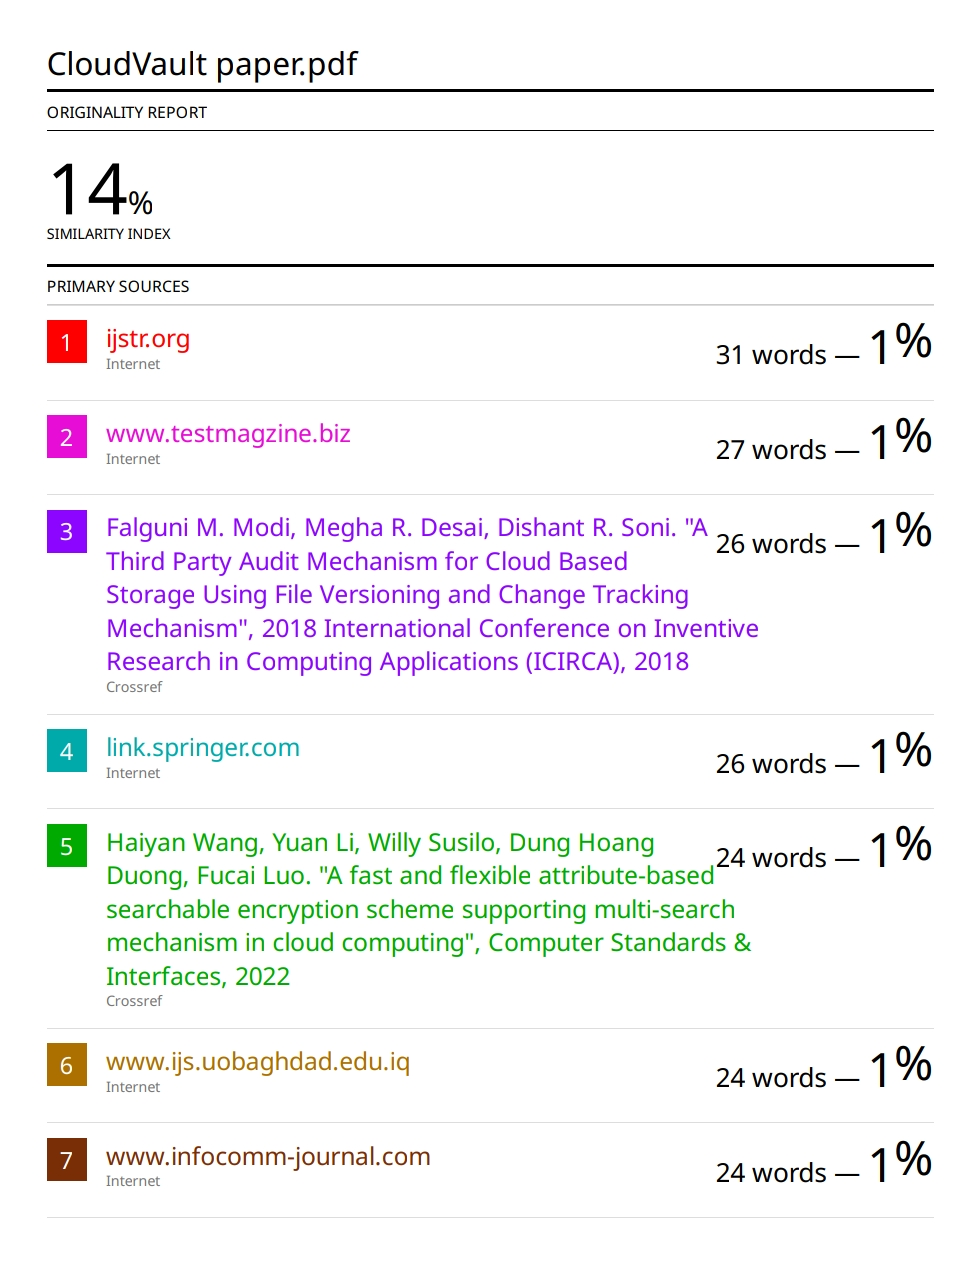
\includegraphics[height=135mm,width=105mm]{Images_Cloud/Plag1.jpg}}
  \caption{Plagiarism}
\end{figure}


\begin{figure}[h]
\section{Activity Chart}
  \centering
  \fbox{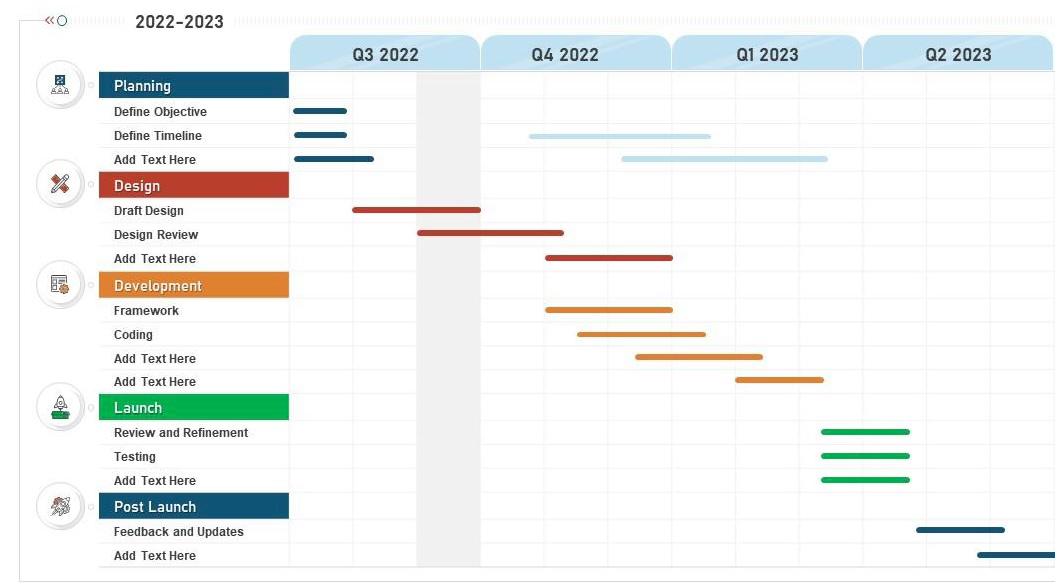
\includegraphics[height=135mm,width=105mm]{Images_Cloud/Activity_chart.png}}
  \caption{Activity Chart}
  \label{fig:performance_comparison}
\end{figure}